\subsection{Symbolic Links}

When exporting the configuration file, it was observed that \gls{cpe} 5 simply writes it in a path on the filesystem. Then the user can download it just by knowing its name, this is also true for any file under the specified directory.

Recently, it was discovered that some residential gateways have a vulnerability that allowed an attacker to access all files of the device’s file system by plugging a flash drive with a symbolic link to root on it \cite{cve-2020-5795}. This allowed the configuration files and password hashes to be recovered by accessing its sharing.

Similarly, a symbolic link to root was placed in the same folder as the configuration exports are stored. The result was that the \gls{http} server follows the symbolic link and allows every file on the equipment to be downloaded, as shown on Figure \ref{figure:cpe_symlink}.

\begin{figure}[h]
    \centering
    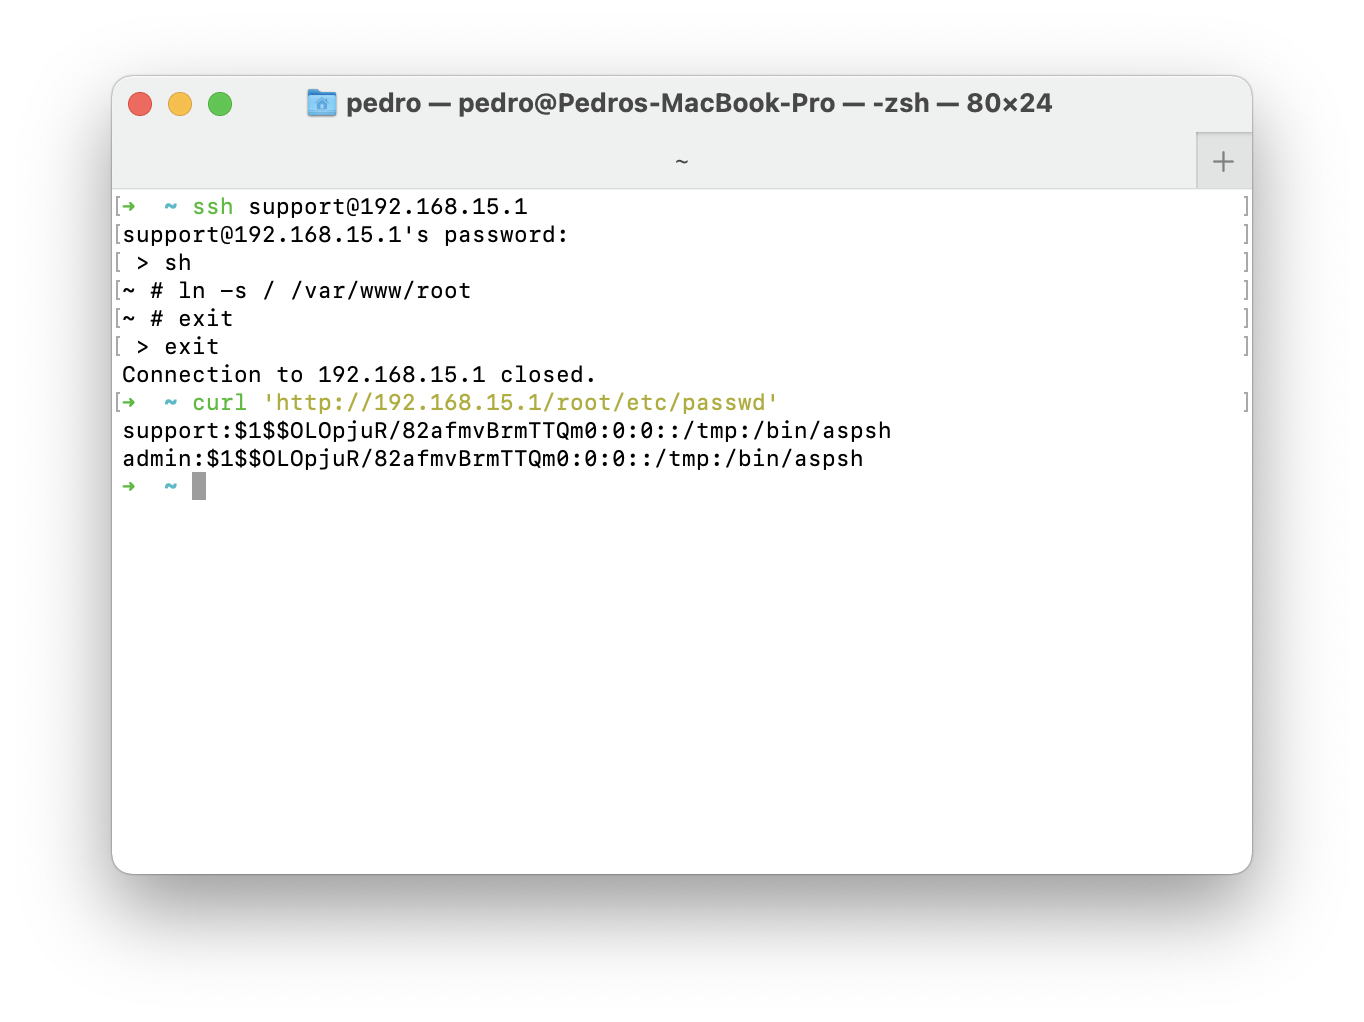
\includegraphics[width=\linewidth]{contents/http-management-interface-analysis/symbolic-links/cpe-http-management-interface-following-symbolic-link.png}
    \caption{\gls{cpe} \gls{http} Management Interface Following Symbolic Link}
    \label{figure:cpe_symlink}
\end{figure}

Although no way of injecting the malicious symbolic link on the device without requiring proper credentials was found, another vulnerability can be discovered in the future that would make this possible. Allowing an attacker to exploit it and gain access to all files on the device, including plaintext credentials.

\FloatBarrier
